\documentclass[a4paper, 12pt, hidelinks]{article}

\usepackage[natbibapa]{apacite}
\bibliographystyle{apacite}
\usepackage{blindtext}
\usepackage{booktabs}
\usepackage{caption}
\usepackage[ddmmyyyy]{datetime}
\usepackage{enumitem}
\usepackage{eurosym}
\usepackage{fancyhdr}
\usepackage{fontspec}
\usepackage[margin=1in]{geometry}
\usepackage[toc,acronym,nonumberlist]{glossaries}
\usepackage{graphicx}
\usepackage{hyperref}
\usepackage[nottoc,notlot,notlof]{tocbibind}
\usepackage[table,dvipsnames]{xcolor}
\usepackage{url}
\usepackage{verbatim}
\usepackage{pdflscape}
\usepackage{epstopdf}
\usepackage{tabularx}
\usepackage{minted}
\usepackage{todo}
\usepackage{pdfpages}
\usepackage{multirow}
\usepackage{subcaption}
\usepackage{fancyvrb}

\setmainfont{Arial}
\pagestyle{fancy}
\renewcommand{\headrulewidth}{0pt}

\lhead{Joe Barrett - 40117680}
\rhead{SOC10101 Honours Project}
\lfoot{}
\cfoot{}
\rfoot{\thepage}

\makeglossary
\loadglsentries{glossary}

\newlist{chapterList}{enumerate}{1}
\setlist[chapterList]{label=\bfseries Chapter \arabic* - }
\newenvironment{where}{\noindent{}where\begin{itemize}[label={}, nosep]}{\end{itemize}}

\begin{document}
	\urlstyle{same}
	\pagenumbering{roman}
	\setcounter{secnumdepth}{4}
	\setcounter{tocdepth}{3}
	\begin{titlepage}
	\begin{center}
		
		\vspace*{3cm}
		{\LARGE Calculation of Mountain Bike Suspension Settings through Image Analysis}
		
		\vspace{3cm}
		{\large Joe Barrett - 40117680}

		\vfill
		Submitted in partial fulfilment of the requirements of Edinburgh Napier University for the Degree of BEng (Hons) Software Engineering
		
		\vspace{1cm}
		School of Computing
		
		\vspace{1cm}
		\today
	\end{center}
\end{titlepage}
	\thispagestyle{empty}
\section*{Authorship Declaration}
I, Joe Barrett, confirm that this dissertation and the work presented in it are my own achievement.
\\\\
Where I have consulted the published work of others is always clearly attributed.
\\\\
Where I have quoted from the work of others, the source is always given. With the exception of such quotations this dissertation is entirely my own work.
\\\\
I have acknowledged all main sources of help.
\\\\
If my research follows on from previous work or is part of a larger collaborative research project I have made clear exactly what was done by others and what I have contributed myself.
\\\\
I have read and understand the penalties of academic misconduct.
\\\\
I also confirm that I have obtained informed consent from all people I have involved in the work in this dissertation following the school's ethical guidelines.
\vspace{2cm}\\
Signed:
\vspace{2cm}\\
Date:
\vspace{2cm}\\
Matriculation Number:
\newpage
\thispagestyle{empty}
\section*{Data Protection Declaration}
Under the 1998 Data Protection Act, The University cannot disclose your grade to an unauthorised person. However, other students benefit from studying dissertations that have their grades attached.
\\\\
Please sign your name below one of the options below to state your preference.
\vspace{3cm}\\
The University may make this dissertation, with indicative grade, available to others.
\vspace{3cm}\\
The University may make this dissertation available to others, but the grade may not be disclosed.
\vspace{3cm}\\
The University may not make this dissertation available to others.
\newpage
	\setcounter{page}{1}
	\begin{abstract}\noindent
		With some mountain bike suspension units costing upwards of £1000, it is vital that they are correctly set up to the rider's weight and riding style. An improper setup can result in damage to the suspension unit and/or injury to the rider. The most basic setting which should be set for every rider is sag, this is the amount the suspension sits into its travel under normal load. Calculated from a percentage of the shock's stroke, setting sag requires knowledge of suspension and repeated measurements which beginner mountain bikers may not know about.
		\\\\
		Image analysis techniques are capable of measuring objects in images computationally without interfering with the subject. By researching the concepts of mountain bike suspension along with the various image analysis techniques and their uses, this project devised an application which could calculate a sag setting for rear suspension with minimal knowledge and input from the rider.
		\\\\
		The application produced was written in Python as it allows for simple use of the chosen imaging library OpenCV. By supplying two images of the rear shock at different pressures, the desired sag percentage, and the shock's stroke length this application is capable of outputting a pressure setting for a baseline setup. By using various evaluative techniques it was proven that the application functions correctly, the results are reliable, and it would be well received by the industry. This application also presents the groundwork for additional projects to extend the functionality and migrate to a mobile platform.
	\end{abstract}
	\clearpage
	\tableofcontents
	\clearpage
	\listoftables
	\clearpage
	\listoffigures
	\clearpage
	\listoflistings
	\clearpage
	\section*{Acknowledgements}
	\todo{write acknowledgements}
	\clearpage
	\pagenumbering{arabic}
	\subsection{Context}
	The suspension on a mountain bike plays a vital part in the rider's performance, comfort and overall enjoyment of the sport. With some suspension units costing upwards of \pounds1000 it is vital that they are setup to function correctly. The objective of this thesis is to research the characteristics of mountain bike suspension, look at methods and applications of image analysis, and produce a prototype mobile application which utilises image analysis to aid the user in setting up their suspension.
\subsection{Background}
	A survey carried out by the International Mountain Bike Association shows the average price of mountain bikes owned in Europe to be \euro2546 (\pounds2206) \citep{imbasurv}. Starting at approximately \pounds1000 \citep{giantstance}, enthusiast level mountain bikes can be purchased with suspension for both the front and rear wheels, known as \gls{fs} bikes whereas \gls{ht} bikes have only front suspension; this difference can be seen in figure \ref{fig:fsandht}. Even at this comparably low cost, the suspension units have multiple adjustments available to optimize and personalize how they operate.
	\begin{figure}[h!]
		\centering
		\begin{minipage}{0.45\textwidth}
			\centering
			\includegraphics[width=8cm]{../images/2017_GIANT_FATHOM_1.jpg}
		\end{minipage}\hfill
		\begin{minipage}{0.45\textwidth}
			\centering
			\includegraphics[width=8cm]{../images/2016_Giant_Reign_Advanced_275_0.jpg}
		\end{minipage}
		\caption{Hardtail and full suspension mountain bikes \citep{giantfathom,giantreign}}
		\label{fig:fsandht}
	\end{figure}
	\\
	To ensure the \gls{fork} and \gls{shock} function correctly they must be set up for the rider's weight and intended use of the bike. As this is considered a specialist area, many entry and mid level riders will lack the knowledge of this process or be unsure of how the suspension should operate meaning the rider could use the bike with the suspension set up incorrectly.
	\\\\
	It has been proven that using a \gls{fs} over a \gls{ht} offers a performance advantage to the rider \citep{fullsusperf}. However if the suspension fork and/or shock have not been set up, it can be detrimental to the rider's performance and potentially lead to injury. For example, if a shock has too little \gls{rebounddamping} set and the rider goes off a jump, the excessive speed at which the rear of the bike extends can create forwards rotation, causing the rider to go over the handlebars of the bike.
	\\\\
	Additionally, an incorrect suspension setup can cause excessive wear and tear on the bike's frame and components. Suspension which is set too soft can allow for bottoming out which expends excess forces into the frame and potentially cracks the frame's structure. Suspension set too hard forces energy, which it would normally soak up, into the wheels and tires causing denting and warping of the wheel rims. Further effects of suspension setup will be explained in following sections.
	\\\\
	Many bicycle retailers will set up the suspension on a newly purchased mountain bike for the customer on delivery. Most of the time this will be enough to avoid incident but due to the extra weight of the equipment riders use, i.e. helmet, hydration pack, body armor which the customer will not be wearing at the time of delivery, this setup is regularly inaccurate. Furthermore, with some manufacturers choosing direct sales over local retailers \citep{roseonline, ytonline}, this setup can be circumvented altogether.
	\\\\
	Since the birth of the modern smartphone in 2007 brought along by the first generation Apple\textregistered\ iPhone\textregistered\ and introduction of the Android\texttrademark\ mobile operating system, the use of mobile computing in everyday life has grown rapidly. Google\texttrademark\ stated that there were approximately 1.4 billion active Android users worldwide in 2015 \citep{androidusers}.
	\\\\
	The introduction of activity tracking devices and mobile applications such as FitBit \citep{fitbit} and Strava \citep{strava} and their growing popularity \citep{apppopularity} shows that individuals are welcome to the idea of using smartphones to aid or augment their participation in hobbies or sports. Due to this popularity and in a bid to give every rider the ability to setup and tune their own suspension, either at home or while out on a ride, companies started producing small devices \citep{sussmybike, shockwiztrademark} and mobile applications \citep{foxird} which aid riders in the process.
\subsection{Aims and Objectives}
	\todo{Revise aims and objectives}
	The aim of this project is to create a prototype application capable of providing the user with a suggested suspension setup using image analysis techniques. This will be achieved by meeting the following objectives:
	\begin{itemize}
		\item Complete a literature review of mountain bike suspension and image analysis techniques including uses of image analysis in sports science.
		\item Design the prototype application
		\item Implement the prototype application 
		\item Evaluate the success and appropriateness of the produced application 
	\end{itemize}
\subsection{Restrictions}
\todo{Write project restrictions section}
\subsection{Thesis Structure}
\todo{Finish structure section}
\begin{itemize}
	\item[Introduction] Outlines the context of the project and states the major aims and objectives
	\item[Literature Review] 
	\item[Methodology]
	\item[Critical Evaluation] 
	\item[Conclusion]
\end{itemize}
	
	\clearpage
	\section{Literature Review}\label{sec:lit_review}
	The aim of this project is to produce an application that makes use of image analysis techniques to provide the user with a suggested set-up for their suspension units. This literature review will identify the intricacies involved in correctly configuring a rear suspension unit and how these make it difficult for riders to do it themselves. It will then go on to highlight how image analysis is carried out and identify the various techniques that are relevant to this project. This review will shed light on the problem at hand and help identify a viable solution.
	
		\subsection{Mountain Bike Suspension Concepts}
		The purpose of suspension on a mountain bike is to absorb the energy created from riding over features such as bumps and rough terrain encountered along a trail, improving comfort for the rider and allowing them to go faster by maintaining better contact between the tires and the ground. This requires the use of a spring and damper, collectively known as a shock absorber, which allows the wheel to move away from the feature on contact and make a controlled return once it has been passed.
	\subsubsection{Travel and Stroke}
		\Gls{travel} is the distance which the bike’s fork or frame allow the wheel to move in an upward direction while \gls{stroke} is the distance that the shock absorber can compress before it bottoms out. \Gls{travel} is measured in millimetres or inches and can range from 80mm to 210mm or 4in to 9in. Bikes designed for different disciplines require differing amounts of travel with those designed for cross-country riding typically requiring less travel than those designed for more aggressive disciplines such as downhill racing having more. See Table \ref{tab:travel} for typical specifications.
		\begin{table}[h!]
		\centering
		\caption{Table of common suspension \glspl{travel} and intended disciplines}
		\label{tab:travel}
		\begin{tabular}{|c|cccc|}
			\hline
			Travel (mm)&Cross Country&Trail&Enduro&Downhill\\
			\hline
			80&\cellcolor[gray]{0.5}&&&
			\\
			100&\cellcolor[gray]{0.5}&&&
			\\
			120&\cellcolor[gray]{0.5}&\cellcolor[gray]{0.5}&&
			\\
			140&&\cellcolor[gray]{0.5}&\cellcolor[gray]{0.5}&
			\\
			160&&&\cellcolor[gray]{0.5}&
			\\
			180&&&\cellcolor[gray]{0.5}&\cellcolor[gray]{0.5}
			\\
			+200&&&&\cellcolor[gray]{0.5}\\
			\hline
		\end{tabular}
	\end{table}
	\begin{figure}[h!]
		\centering
		\includegraphics[width=12cm]{../images/reignschpath.PNG}
		\caption[Diagram showing travel and stroke on a full suspension bike]{Diagram showing 
			travel and stroke on a full suspension bike\footnotemark}
		\label{fig:travelvsstroke}
	\end{figure}
	\subsubsection{Front Suspension}
		Front suspension commonly employs a linear telescoping shock absorber, known as a \gls{fork} due to it's dual sided construction. On nearly all suspension \glspl{fork} the \gls{stroke} is 1:1 with the potential travel of the wheel. Front suspension is found on 
		all \gls{fs} and \gls{ht} bikes.
	\subsubsection{Rear Suspension}\label{sec:lit_review_rear_suspension}
		Rear suspension uses a shock absorber that is much shorter than a fork so it cannot operate on a 1:1 ratio and still allow the desired travel. Full suspension frames incorporate one or more pivot points and linkages which allow the wheel to move and act as multipliers for the suspension. Rear ratios are expressed as n:1 where n is the average distance the rear wheel moves for every 1mm the shock compresses throughout its stroke; the leverage ratio changing constantly across the compression cycle.
		\\\\
		The difference between front and rear stroke and travel can be seen in Figure \ref{fig:travelvsstroke} noting the separation of rear wheel travel from the stroke of the shock absorber. Although manufacturers design their rear suspension differently, the rear wheel always rotates around the main pivot, (or in some cases a virtual pivot), as opposed to moving linearly as front forks do. As a result, the frame behaves differently through its travel, depending on the number and location of pivot points and the type of shock that it is being used. 
		\\\\
		Because of this the average ratio is normally dismissed in favour of a leverage curve that plots the ratio n:1 throughout the compression cycle. Figure \ref{fig:3_bike_lev_ratio} shows the leverage curves of three modern suspension designs. Each of these designs has between 150mm and 170mm of travel and uses the 27.5 inch wheel size. However, it is evident that varying the location of pivot points produces suspension with drastically different characteristics.
		\begin{figure}[h!]
			\centering
			\includegraphics[width=10cm]{../images/3_bike_lev_ratio.jpg}
			\caption{Leverage curves of three modern suspension designs}
			\label{fig:3_bike_lev_ratio}
		\end{figure}
		\\
		The Virtual Pivot Point (VPP) design of the Giant Reign (shown blue) has an initial falling rate, meaning the shock can be compressed easily, but slows down and even rises slightly towards the end of its travel as seen in Figure \ref{fig:3_bike_lev_ratio}. This means the suspension will feel soft most of the time but stiffer as compression increases. This is emphasised by the Horst link system of the Lapierre Spicy (shown magenta) where the leverage curve rises significantly towards the end of its travel.In contrast, the curve of the single pivot Empire MX-6 Evo (shown green) is effectively linear. This is due to the MX-6 having only one pivot and swinging arm, as opposed to multiple pivots and linkages of the VPP and horst link designs, so there is an almost direct input from the rear wheel to the shock. The physical differences in each of these frames can be seen in Figure \ref{fig:3_bike_diagrams}.
		\begin{figure}[h!]
			\centering
			\begin{subfigure}[t]{0.3\textwidth}
				\centering
				\includegraphics[width=\textwidth]{../images/3_bikes/giant.png}
				\subcaption{Giant Reign}
			\end{subfigure}
			\begin{subfigure}[t]{0.3\textwidth}
				\centering
				\includegraphics[width=\textwidth]{../images/3_bikes/empire.png}
				\subcaption{Empire MX6 Evo}
			\end{subfigure}
			\begin{subfigure}[t]{0.3\textwidth}
				\centering
				\includegraphics[width=\textwidth]{../images/3_bikes/lapierre.png}
				\subcaption{Lapierre Spicy}
			\end{subfigure}
			\caption{Full suspension frame comparison}
			\label{fig:3_bike_diagrams}
		\end{figure}
		\\
		For this project two bikes will be used for development and testing of the application. The first is a 2015 Giant Reign, shown on figure 3 in blue, as it will be constantly available throughout the project. The frame uses Giant’s Maestro™suspension system which is a variation of VPP. Like all VPP systems Maestro uses two links, an upper and lower, to create a virtual main pivot point, however unlike other VPP systems, Maestro creates its virtual pivot as close to the rear of the frame as possible As shown by the red circle in Figure \ref{fig:maestro}. The second will be a 2011 Orange 5 which has the same suspension design as the Empire MX6 Evo in Figure \ref{fig:3_bike_lev_ratio}. This bike was selected as it has a completely different design to the Giant Reign and will also be easily accessible throughout the project. 
		\begin{figure}[h!]
			\centering
			\includegraphics[width=12cm]{../images/reignsch.PNG}
			\caption{Maestro suspension}
			\label{fig:maestro}
		\end{figure}
		\\
		Although rear suspension designs are complex, neither the average rider nor professionals, such as mechanics, working in the industry necessarily need this specialist knowledge. Leverage curves are predominantly used by designers to determine how a particular suspension unit will behave when researching and designing new frames \citep{creek2016curves}. Though having an understanding of leverage curves will help the individual rider to fine tune their suspensions settings described in the following sections themselves, the majority will take little interest in the differences between a single pivot and VPP design, choosing a simpler ”set and forget” approach to their suspension. 
		\\\\
		In the context of this project and the intended user for the application, this begs the question of how much information should be provided to the user? Modern human /computer interaction principles aim toward providing information to the user which is relevant and necessary in context \citep{shneiderman2010designing}. Presenting the user with a leverage curve which may require extensive interpretation before they understand the implications within the limitations of a mobile application may prove detrimental to the user experience. For an application which is intended to remove the difficulties of suspension setup and allow for quick and easy production of a basic setup, providing a single sag setting would be preferable over a plethora of of technical data.	
	\subsubsection{Sag} \label{sec:sag}
		\todo{review section adding detail on setup method}
		Sag is the amount that the suspension sits into its travel when the rider is in a neutral position, described in Figure \ref{fig:sag}. It is required so that the suspension has travel available to extend as well as just compress and is calculated using the rider’s weight, available travel, and intended riding style.
		\\\\
		The amount of sag depends on the stiffness of the suspension unit which can be adjusted by changing the air pressure of an air spring or replacing the spring and adjusting the preload of a traditional coil shock. Depending on discipline and the	amount of travel the bike has, sag can vary between 15\% and 40\% of the available travel though it is typically set at between 25\% and 35\% for the average rider with greater variances only encountered in competition.
		\begin{figure}[h!]
			\centering
			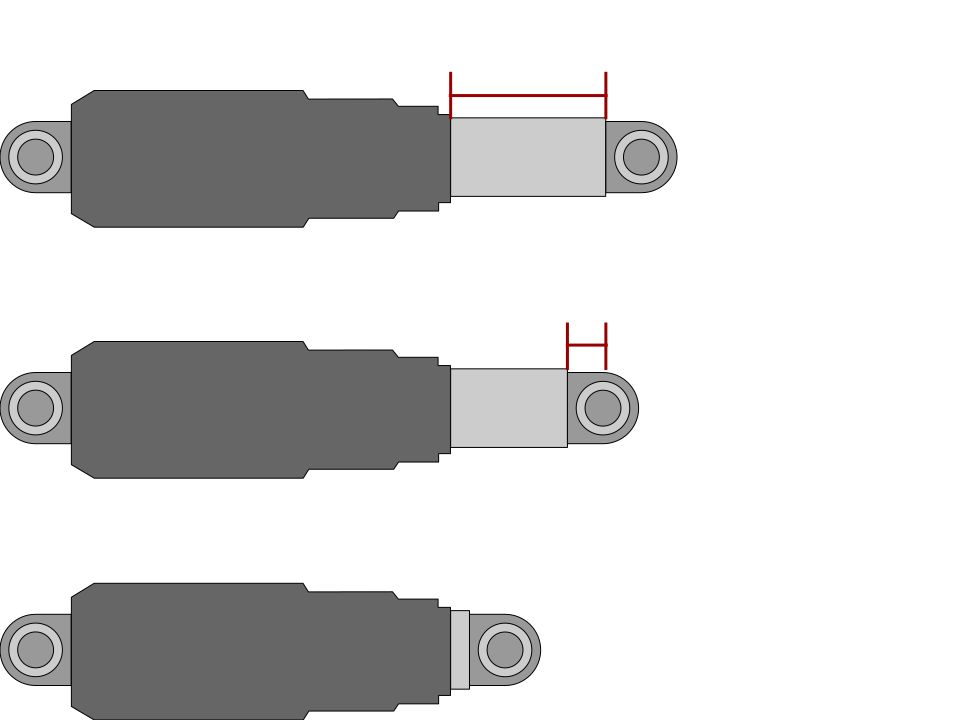
\includegraphics[scale=0.5]{../images/sag_diagram.png}
			\caption{Diagram of shock states indicating sag}
			\label{fig:sag}
		\end{figure}
		\\
		Sag is set by first calculating the distance that the shock should sit into its travel by producing the desired percentage of the shocks stroke. For an air shock the manufacturers recommended pressure is then pumped into the shock and the rider weights the bike. On each air shock there is a marker o-ring which is pushed down the shock shaft when the shock is compressed. The position this o-ring ends at can be measured and the shock pressure adjusted accordingly until it sits at the target measurement. 
	\subsubsection{Damping}
		In a spring and mass system, when the spring is elongated it will exert a returning force on the mass which, according to Hooke's law \citep{rychlewski1984hooke}, is directly proportionate to the distance which the spring has been pulled. In suspension this force is explained as two separate forces. If an individual were to push down on mountain bike suspension they would feel a resistance, this is known as compression, and when they let go the suspension will return to its neutral state, this is rebound. Both of these can be controlled which is known as damping.
		\\\\
		Suspension damping works by forcing oil within the shock absorber through a series of holes in the absorber’s damping circuit. Reducing the size or number	of holes increases resistance, reducing the speed at which the oil flows through the circuit to increase the damping effect by making compression and rebound slower.
	\paragraph{Compression Damping} 
		This is applied while the shock absorber is being compressed to control the effort required to do so. Increasing damping forces the wheel to remain in contact with the ground which makes the suspension feel stiffer. However too much compression damping can make the suspension overly stiff so it does not effectively absorb the impact of bumps and rough terrain. Conversely, too little compression damping can cause the suspension to ”blow through” all of the available travel prematurely with nothing left to soak up impact when it is most required. 
	\paragraph{Rebound Damping}
		This is used to control the speed at which the shock absorber recovers to its normal riding position after compression. An optimal setting will allow the suspension to track the ground, quickly and smoothly returning to the correct position after a bump or hole is passed. 
		\\\\
		Too much rebound damping causes the suspension unit to recover slowly and sometimes “pack down” meaning the shock absorber remains compressed for too long leaving the rider fully exposed to the next impact. Too little rebound damping can cause the suspension to “buck” the rider, like a horse, and potentially cause an accident.
	\paragraph{High and Low Speed Damping} 
		The ways of adjusting compression and rebound damping differ by manufacturer and model with better specified bikes having two adjustable speeds for each damping circuit giving four damping settings. High speed adjustments are used in high G-force situations such as riding large jumps or drops where compression needs to be set softer to absorb impacts and rebound set slower so the rider has time to recover without the equilibrium of the bike being upset.
		\\\\
		Low speed damping set ups are used against lower G-force movements such as rider weight shifts or long, slow compressions. Optimally compression is set stiffer as this type of feature can use a lot of travel and rebound damping set faster to deal with multiple features in quick succession.
	\subsubsection{Optimal Setup}
		Although setups will vary between rider, suspension system and discipline, there are some key principles that all riders should aim to achieve. Sag should be set to an appropriate measurement by adjusting the air pressure on air shocks or spring rating on coil shocks. Compression damping should feel soft and soak up bumps efficiently without excessive bottoming out. Rebound damping should be set to return as fast as possible without bucking the rider, which is normally somewhere in the middle of the two setting available with a slight bias towards the faster option.
		\\\\
		Attaining this optimal setup can be difficult for both beginners and intermediate riders as they lack experience and in-depth knowledge of suspension units and may not know how different frames react while being ridden. Knowing which measurements to make and the calculations required to correctly configure sag, compression and rebound settings are typically beyond the capabilities of this level of rider unless they have been previously trained by a professional or investigated the topic in detail for themselves.
	\subsection{Image Analysis}
	\gls{ia} is the use of various techniques, such as pattern recognition, geometry calculations, and signal processing, to extract information from digital images. Image processing is the application of various processes on an image to change or enhance its appearance. In practice, the processing stage normally comes before the analysis stage as a way of simplifying the image prior to analysis in order to maximize the likelihood of obtaining usable data.
	\subsubsection{Digital Camera Operation}
		A digital camera operates by capturing visible light reflected by objects onto the camera’s sensor. The light must travel from the object through a convex focusing lens which refracts the light onto a corresponding point on the sensor.
		\begin{figure}[h!]
			\centering
			\includegraphics[width=10cm]{../images/camera_bulb.PNG}
			\caption[Diagram of camera and lens operation]{Diagram of camera and lens operation \citep{introtoprocessing}}
			\label{fig:camera_diagram}
		\end{figure}
		\\
		The distance between where light enters the lens and the point at which it is no longer diffused is known as the focal length, marked $f$ in figure \ref{fig:camera_diagram}. This point can be adjusted by changing the optical characteristics of the lens so that the refracted light hits the sensor to create a sharply focused image.
		\\\\
		A camera’s sensor is made up of an array of photosensitive cells capable of collecting light and generating an integer value based on the brightness and colour of the received light. The microprocessor inside the camera takes these values and converts them into the image data, sometimes taking an average of the surrounding values to better understand the light as it was captured. Each of the cells in the camera’s sensor equates to a single pixel in the final image. For example, a camera with a sensor made up of 1920 cells across by 1080 down (otherwise known as a 2 megapixel sensor) produces an image 1920 pixels wide and 1080 high. The larger the physical size of the sensor, the more cells it can contain resulting in a higher quality image.
		\\\\
		Image processing is the manipulation of these integer values to adjust the visual appearance of the image for either artistic or scientific purposes. Image analysis is the comparison of these values either to their neighbours or in clusters to locate features, produce measurements, or for other purposes within the context of the image.
	\subsubsection{Lighting Conditions}
		When capturing images to be analysed, it is important to have good lighting conditions so that none of the required detail is lost \citep{introtoprocessing}. If the image is captured in unsuitable conditions, such as low light, then this can seriously affect the outcome of subsequent analysis. 
		\\\\
		Certain image processing techniques, such post-processing images captured as Camera RAW files, can help ameliorate poor lighting conditions though this is not foolproof and it is always better to capture a well-lit image. Figure \ref{fig:illumination} shows the effects that different lighting angles have on a subject.
		\begin{figure}[h!]
			\centering
			\includegraphics[width=\linewidth]{../images/face_illumination.png}
			\caption[]{The effects of different lighting conditions on a face \citep{introtoprocessing}}
			\label{fig:illumination}
		\end{figure}\\
		It can be seen that the situation which highlights the most detail is when the light source is close to being in front of the subject matter. Such lighting reduces the amount of image processing required before analysing and produces the largest amount of usable data. In the context of this project many smartphones also have an integral flash function which means the user can correctly light their image in sub-optimal lighting conditions where required detail may otherwise be lost.
	\subsubsection{Usages}
		Image processing and image analysis have been applied to multiple areas with its value and effectiveness rapidly improving alongside advances in camera technology and computing power. These applications range from facial recognition in social media uploads \citep{zuckerberg2011tagging} to the utilisation of satellite imagery to track the changing shape of coastlines \citep{costalimagery}.
		\begin{figure}[h!]
			\centering
			\includegraphics[width=15cm]{../images/4panel.png}
			\caption[Uses of image analysis]{Uses of image analysis, from top left clockwise: An MRI brain scan, automotive night vision with pedestrian recognition, infrared image taken with a smartphone, chemical rock analysis from mars}
			\label{fig:analysis_uses}
		\end{figure}
		\paragraph{Medical}
			This is arguably one of the most important uses of IA. Advances in medical imaging have reduced costs, diagnosis time and patient recovery time while improving the ability to localise and personalise treatments \citep{esfmedical}. Major uses of IA in medical applications are the use of Magnetic Resonance Imaging (MRI) and Computerised Topography Scanning (CT Scan) to create detailed images of the human body and identify illness before obvious symptoms appear. This is shown top left in Figure \ref{fig:analysis_uses}.
		\paragraph{Transport}
			Image analysis has been included in the consumer automotive market on various models since 2004 when Honda introduced a thermographic night vision camera with automatic pedestrian detection on their Legend model \citep{hondanightvision}. Other manufacturers, including Audi, have since introduced similar technology and their implementation can be seen top right in Figure \ref{fig:analysis_uses}. Since this initial use many other vehicle manufacturers have included functionality based on image analysis expanding its use into areas such as the automatic recognition of speed limit signs, lane departure warning systems, and automatic braking systems based on hazard recognition.
		\paragraph{Engineering}
			The use of image analysis in engineering has helped to create more stable and efficient structures, in bridges and skyscrapers for example, by looking at the materials used in their construction \citep{concreteanalysis} and monitoring their stresses and potential areas of weakness \citep{bridgecables}. Today advances in mobile computing have allowed engineers to routinely use IA while on site and some application vendors target their products at an engineering sector by improving their durability and integrating features such as infrared imaging \citep{catphone}, the output of which can be seen lower right in Figure \ref{fig:analysis_uses}.
		\paragraph{Space}
			While some industries make use of satellite imagery to monitor 
			chan-ges to our own planet, agencies such as NASA and ESA use image analysis to look at other planets and celestial bodies. The Martian rover, Curiosity, uses multiple cameras for navigation, hazard avoidance, and scientific imaging with the images streamed back to Earth for detailed analysis. Major uses of such extraterrestrial images include the identification of geological formations and their likely composition \citep{curiositysand, curiositygravel} and the location and identification of chemicals using the analysis tools such as ”ChemCam” \citep{curiosityhydrogen}, which can be seen lower left in Figure \ref{fig:analysis_uses}.
	\subsubsection{Image Analysis Techniques}
	There are multiple techniques which can be applied to imagery to produce a variety of outcomes or further prepare images for additional analysis such as custom algorithms. 
	\paragraph{Edge Detection}
	\paragraph{BLOB Analysis}
	\paragraph{Taking Measurements}
	\subsection{Image Analysis in Sports Science}
	The benefits of image analysis in sports science are most prevalent in the area of biomechanics. In most sports , an individual’s performance depends on a combination of physical fitness and skills. In certain sports, such as motorsports \todo{cite}, equipment is undeniably important although unless “driver-athletes” can cope with the stresses and strains of race conditions they are unlikely to achieve success regardless of the technical superiority of their vehicle.
	\\\\
	In such sports, the performances of cars, motorcycles, and even mountain bikes are all predictable and measurable. They have all been designed and manufactured to be as fast as possible within the rules laid down by the sport’s governing body so it is important to continually analyse and fine tune their set – up by changing tires or adjusting suspension to seeking out the margin gains that make the difference between gaining a place on the podium or not. As a result, performance cars and bikes are fitted with an array of sensors that constantly monitor critical aspects of performance \todo{cite}. 
	\\\\
	Fitting sensors to humans without impairing their mobility is not quite so simple. To provide the best testing ground for fitness and technique, the participant should be unhindered and able to perform tasks without data capturing equipment getting in their way. Image analysis can play a large part in this as utilising various techniques can allow for stable and repeatable test situations while also providing a platform for reviewing the captured images. A study into bowling techniques in cricket used a mix of manual point picking and automated measuring from images to produce data such as angle and speed of bowling deliveries as well as ball spin \citep{cricketimaging}. While the dataset was limited due to conflicts with the players’ training schedules, the results proved useful and were subsequently replicated in a pitching machine so that batsmen practised against more lifelike deliveries.
	\\\\
	A second study on the use of IA in showjumping \citep{jumpyhorses} made use of techniques similar to those used by Cook, Justham, and West. In this instance, the angles of the horse’s limbs were recorded and compared over a period of four months to analyse whether different training techniques delivered measurable improvements. Here, passive image analysis was chosen as the preferred technique as attaching sensors to the horse could have frightened the animal and almost certainly caused it perform below par.
	\subsection{Image Analysis for Optimizing Mountain Bike Suspension}
	Though image analysis has been used for calculations in many engineering and sports applications \citep{concreteanalysis, bridgecables}, it is relatively unused with mountain bike suspension with only the specialists at Fox Racing Shox using the technology \citep{foxird}. The mobile application that Fox has locks to the forks and shocks that the company manufacture although the image analysis techniques they use are adaptable enough to be used on suspension units from other manufacturers. 
	\\\\
	By harnessing the image capturing and computing power of modern smartphones, image analysis can be applied to mountain bike suspension to produce a simple method of calculating a baseline setup for any suspension unit. The measurements and calculations required can be removed from the user’s responsibility to create a simple and efficient method of generating a safe and reliable suspension setup.
	\subsection{Conclusion}
		By identifying the key aspects and settings relating to mountain bike suspension and the common image analysis techniques, this literature review has highlighted the processes that this project can utilise to achieve its aims. By using this knowledge, the following sections will identify distinct methods which the project could use and cover the results of how the application performed under test conditions.
	\clearpage
	\section{Methodology}\label{sec:methodology}
	\subsection{Introduction}
		This chapter gives an outline of the methodologies used to complete the work identified in the previous chapters as well as the reasons for using these methods and rejecting alternatives that could have been used. The effectiveness of these methods determines the success of the project so those chosen need to be both reliable and manageable. A technical approach was identified for the most appropriate way to produce a solution to the problem identified and a project management approach was decided on so that the project could remain on track and meet the required deadline.
	\subsection{Literature Review}
		The purpose of the literature review presented in section \ref{sec:lit_review} of this dissertation is to outline, investigate, and clarify the subject areas with which this project is involved. This aids both the reader and author in understanding these subject areas and helps to explain how the project presents a viable solution to the problem area.
		\\\\
		There are numerous forms a literature review can take although not all have the same aims. A traditional or narrative review can be carried out to critique a body of literature and potentially locate inconsistencies \citep{adams2007research}. This type of review is normally used when the research question is well defined. Alternatively a systematic literature review can be undertaken although this requires a more rigorous process and takes more time. Systematic reviews aim to locate previous studies that are within the same or similar subject areas and gain insight to expedite answers to the questions presented by the research \citep{kitchenham2009systematic}.
		\\\\
		For this project a combination of both methods has been used. A systematic approach was applied to investigate how image analysis is used and ascertain which particular techniques were relevant to the use of IA in the context of mountain bike suspension. A traditional method has been applied to examine the uses of image analysis in sports science to determine whether previously used techniques would transfer to mountain bike suspension and provide some idea of how effective they could be.
		\subsubsection{Source Selection}
			Regardless of which types of review was chosen, it was necessary to adopt a methodological approach to identify sources relevant to the project. Multiple services are available for viewing academic papers online and for this project the Edinburgh Napier University library and Google Scholar were utilised as between them they provide an expansive library to select from using a variety of advanced search filters.
			\\\\
			As the  application of advanced technologies to mountain bike suspension is in its infancy and commercially driven, much of the research is undertaken by the manufacturers themselves so there were no academic sources to use. As a result, numerous multiple mountain bike websites and blogs have been cited. In a subject area where the research is more established this would be frowned upon as such sources tend to be biased and often unproven. However it was entirely unavoidable.To overcome author bias, multiple sources have been cited wherever possible as a way of providing different viewpoints on the same topic.
			\\\\
			To determine whether a source is suitable requires a methodical and critical approach. Even before reading a paper or article, it is possible to decide whether the subject matter and research is up to date by referring to its publication date. Such an approach was adopted for this project in order to identify the most recent research available. As a second step, online libraries provide metrics about the number of times a paper has been cited elsewhere; the inference being that papers that have been cited most are both more relevant and trustworthy. However, applying this rule of thumb needed care as some papers are cited so frequently purely because they are the most controversial. Finally when reading a paper, the abstract should be read first followed by the conclusions. This takes little time and taken together, the abstract and conclusions provide a good indication of whether the paper contains relevant and reliable research. Only then should the body of the paper be read in its entirety. 
	\subsection{Platform}
		As a proof of concept, the final product of this software project could take a variety of forms. In line with current products on the market, an application for Android could be produced which would demonstrate the capabilities of image analysis on a mobile device. Alternatively, the image analysis algorithm can be produced in the Python programming language as a script creating a simpler prototype but clarifying the solution that is the core of the problem.
	\subsubsection{OpenCV}
		OpenCV is an open-source computer vision library created for a variety of platforms. Originally released by Intel in 1999 \citep{bradski2008opencv} the library was intended as a research project to aid in CPU intensive visual applications. In 2012 the library was taken over by OpenCV.org \citep{opencvsite}, a non-profit organisation who provide support and documentation. Although the library is written in C and C++, modules are available for Python, Fortran, and the Android platform.
		\\\\
		This project will use OpenCV as it is widely accepted as the best, free computer vision library available and provides functions for the various processes this project requires. Additionally it is well supported and documented which will aid in the development process.
	\subsubsection{Experimentation}\label{sec:methodology_platform_experiments}
		To further understand what may be required to produce both the Android and Python based approaches and aid in deciding which method to use some basic experiments were carried out to compare the two. For the Android experiments some example applications which are bundled with the OpenCV library were hand copied and run on a mobile device. This allowed their output and functionality to be seen while simultaneously gaining experience in using OpenCV on Android. For the Python based approach, tutorials from the \url{www.pyimagesearch.com} website created by Adrian Rosebrock \citep{pyimagesearch} and the \url{www.pythonprogramming.net} website \citep{pythonprogramming} were followed and run on a desktop computer.
		\\\\
		Appendix \ref{app:android_experiments} shows the experiments which were carried out on the Android platform. It should be noted that, while all applications do not show compilation errors and were adjusted to work with the updated version of Android which the device was using, only two of the four experiments worked successfully. Although a stack trace of the errors was produced they do not explain the cause of the error. This is due to how OpenCV works on the Android system.
		\\\\
		Alongside the Android \gls{sdk}, Google provide a \gls{ndk} to allow modules which were not originally written in Java to be run on Android devices. The \gls{ndk} understands various programming languages and applied a Java wrapper around them that is capable of extracting their functionality. This must be applied when using OpenCV on Android as it is written in C++. An artefact of using the \gls{ndk} is that it cannot convert the stack trace produced by errors in the C++ module and following research into this issue it was found that this is difficult to rectify.
		\\\\
		The two working Android experiments do not operate as expected either. Appendix \ref{app:android_experiments} shows the issues with each that were encountered in the test. Although steps were taken to rectify the orientation in the Hello CV experiment and the full-screen issue in both, any fix which was applied was not accepted by the system. Research and debugging of these faults did not rectify these issues to produce an acceptable outcome. Appendix \ref{app:python_experiments} shows the experiments that were carried out using Python. These were much more successful than the Android experiments as they are all functioned and worked exactly as anticipated.
		\\\\
		Appendices \ref{app:android_experiments} and \ref{app:python_experiments} show a comparison between the two methods including the number of files and lines of code required to create the program as well as the relevant source code for each program. There is a clear difference between the two methods. The Android method taking an average of 295 lines of code over 3 files to produce arguably less complex and less functional applications than is produced by Python’s 21 lines of code over 1 file.
		\\\\
		Due to the difficulties encountered when using OpenCV on Android, the decision has been made to produce a proof of concept for the image analysis in Python which also benefits from being an operating system that is already a proven platform for mobile applications. This will allow the project to maintain focus on the analysis and algorithmic side of the solution as opposed to its portability. The decision also allows for more time to be spent making the program functionally stable which will serve as a better demonstration of the solution.
	\subsection{Source Code}
		\subsubsection{Pythonic Coding}
			A metric of software quality is the conciseness and descriptiveness of the source code. The aim of the Python programming language is to complete the same tasks as other object oriented languages but in fewer lines and in a more readable manner \citep{kuhlman2009python}. By removing brackets and instead using indentation to define the boundaries of classes, functions, and conditionals as well as using worded operators, Python creates source code which reads like a list of instructions for people rather than computersas shown in Listing \ref{lst:python_example}. The source code for this project will be written in a pythonic way where it makes sense to do so.
\begin{listing}[ht]
\begin{minted}
[frame=lines,
breaklines,
fontsize=\footnotesize,
linenos]
{python}
long_string = 'This is a very long string'
if 'long' in long_string:
    print 'Match found'
\end{minted}
\caption{An example of Python code}
\label{lst:python_example}
\end{listing}
		\subsubsection{Naming}
			As well as the readability which comes with Python, further efforts will be made to ensure all classes, methods, and variables will be named as descriptively as possible. This makes the system and its algorithms easier for an outsider to understand if any parts of the code need to be revisited at a later date. This is demonstrated in Listing \ref{lst:bad_naming_examples}, where although the left-hand code looks cleaner, when read through looks extremely generic and could be part of any system. In contrast the right-hand code is much more descriptive of its function.
\begin{figure}[!h]
	\begin{minipage}{0.5\textwidth}
		\centering
		\begin{minted}
		[frame=lines,
		breaklines,
		fontsize=\footnotesize,
		linenos]
		{java}
public List<int[]> getThem() {
  List<int[]> list1 = new ArrayList<int[]>();
  for (int[] x : theList)
    if (x[0] == 4)
      list1.add(x);
  return list1;
}
		\end{minted}
	\end{minipage}
	\begin{minipage}{0.5\textwidth}
		\centering
		\begin{minted}[frame=lines,
		breaklines,
		fontsize=\footnotesize,
		linenos]
		{java}
public List<int[]> getFlaggedCells() {
  List<int[]> flaggedCells = new ArrayList<int[]>();
  for (int[] cell : gameBoard)
    if (cell[STATUS_VALUE] == FLAGGED)
      flaggedCells.add(cell);
  return flaggedCells;
}
		\end{minted}
	\end{minipage}
	\captionof{listing}{Examples of bad naming (left) and proper naming (right) taken from Clean Code \citep{martin2009clean}}
	\label{lst:bad_naming_examples}
\end{figure}
	\subsubsection{Object Orientation}
		Object orientation is the use of classes which contain their specific variables and methods to protect functionality from other parts of a system. An object oriented approach will be taken when creating the system to ensure its functions and data is protected should it ever be used as a module elsewhere. The use of private variables and methods with one or two public methods provides an \gls{api} with which other developers can use the system.
		\\\\
		Python does not provide the private and public keywords as found in the Java or C++ languages. Instead it identifies methods and variables prefixed by one or two underscores as protected. This means these items will be hidden from view in autocompletion systems or documentation but remain accessible should the developer require them. The creators of Python chose this method as they enforce responsibility over restriction.
\subsection{Testing}
	To verify the functionality and quality of a software application it must always be tested. This can be carried out at a variety of levels from testing a single class method to an entire system and by knowing how an application works in white-box testing or being unaware of the functionality in black-box testing.
	\subsubsection{Unit Testing}
		Unit testing is carried out on individual units of source code to ensure they are functioning correctly. Normally carried out in the scope of an individual class or module, these unit tests are typically written by the same software developer who produced the class itself. A single unit test comprises of a set-up process where data and objects are initialised, the test itself including an assertion on a variable determining pass or fail, and a tear-down process where any changes to data or memory the test has made are cleaned up.
		\\\\
		As unit tests are simple in structure and quick to run they are commonly executed when changes are made to the source code. This verifies that the changes made have not broken other sections of code and can be committed into the master branch successfully. If a test failure does occur then each unit test should be concise and descriptive enough to aid the debugging process by indicating what has failed and where.
		\\\\
		A metric of quality for unit testing is code coverage. To confirm that a class is of good quality and functional, every possible path through the code must be tested. Testers should aim for 100\% coverage of a module meaning every possible piece of functionality has an associated test with a coverage of 85\% for example meaning that 15\% of a module is not under test and could cause undetected problems if any changes are made. Many integrated developers environments (IDEs) or testing suites provide coverage checking functionality to make this process simple.
		\paragraph{Python Unit Testing}
			Due to the package based and open-sourced nature of the Python programming languages there are many implementations of unit testing frameworks to choose from. Each has its own advantages and disadvantages and there is much debate over which framework is the best to use. A good unit testing framework should provide the necessary functions to create simple unit tests for each path in the source code and be substantial enough to ensure the class or module is correctly tested.
	\subsubsection{Project Testing Scope}\label{sec:project_testing_scope}
		Due to the small size of the application which will be produced in this project, testing will be limited to unit testing as there is no integration to be carried out. This small size also means that 100\% code coverage will be simple to achieve. From this, stability and functionality of the application can be verified improving the quality of the overall product.
		\\\\
		Once the basic functionality has been added to the application, unit tests will be created covering all source code produced including normal operation and sections which can potentially produce errors. This means any subsequent changes can be tested to see if they have affected functionality. Any new functionality will have tests added to the testing suite to maintain 100\% coverage.
		\\\\
		The Python unit testing framework chosen is unittest2. Although it has been superseded by Python3, Unittest is the default framework used by the PyCharm \gls{ide}. The unittest2 module provides a backport of this functionality for use in Python2 meaning extra testing functions are provided to allow more suitable tests to be created. PyCharm also provides the ability to run tests with code coverage producing a clear indication of which sections of source code are covered and which are not. This will be greatly beneficial to achieving full coverage.
\subsection{Project Management}\label{sec:project_management}
	\subsubsection{Agile Development}
		Introduced in 2001 with the writing of the Agile manifesto \citep{beck2001manifesto}, agile development methodologies focus on the rapid delivery of high quality software rather than rigorous design-based structure of traditional waterfall methods. By utilising various techniques such as stand-up meetings, a strong customer focus, and sprint development cycles, agile has become widely adopted in industry and has been proven to produce successful projects that are both more closely tailored to the customers’ needs and delivered in shorter time scales \citep{state_of_agile_2015}.
		\\\\
		There are numerous agile methodologies (XP, Scrum, DSDM) each with their own principles and techniques. However it is commonplace for a company to create their own agile approach picking and choosing items from different methodologies to suit their particular needs \citep{aydin2004agile}. As this is a solo project with no customer then a single set methodology will not be used. Instead a variety of methods may be used to help manage the project and drive the efficiency of the development process. These potential methods will be outlined in the following sections.
		\paragraph{Requirements Analysis}
			Used in some form by the majority of agile methodologies \citep{cao2008agile}, requirements analysis or requirements engineering is a variety of processes used to create the conditions that a project must meet. These requirements take into account stakeholders, users, and the development team or teams. Each requirement should be documented, actionable, measurable, testable, and traceable to aid in its understanding and completion.
			\\\\
			The techniques used to produce requirements include stakeholder identification and interviews which are used to identify what the stakeholders of the project require once it is completed. These interviews may be followed by Joint Requirements Development Sessions which bring stakeholders together to further discuss the requirements of the project. A more traditional approach is to produce a contract-style requirements list although these are typically extensive and incomplete as considerable collaboration is involved in producing them. The requirements analysis techniques that are most frequently used in agile developments are use cases and user stories. These are either written or diagrammatic descriptions of how the system will interact with users or other systems and provide an indication of what will be required from the product.
			\\\\
			Because the application being produced is a prototype and there are no defined stakeholders, the only requirements analysis technique which would be applicable is production of use cases. These can aid in identifying how the application will be operated by users and what the project will need to produce. These requirements can then be prioritised using the MoSCoW format and inserted into a tracking system for the development process as described in the following sections.
		\paragraph{MoSCoW}
			First used in the DSDM agile framework \citep{bittner2002use}, MoSCoW analysis or prioritisation is the process of taking the requirements of a software product and placing them into one of four categories; Must, Should, Could, and Won’t have. These deliverables may then be prioritised either for the entire project or for individual sprint cycles depending on the size and magnitude of the project.
			\\\\
			MoSCoW was created to give customers a better understanding of software requirements. Unlike categorizing priorities as high, medium and low, MoSCoW is more descriptive of what the prioritisation means for the software project. From a development point of view, this prioritisation process allows developers to focus on the core requirements of the project first, creating a viable software solution early in the development cycle with less important features being added later if the resources are available.
			\\\\
			This project could use MoSCoW to prioritise the requirements identified using the requirements analysis technique. This will ensure that the core aspects of the solution are implemented first creating a successful project early and allowing it to improve as time allows.
		\paragraph{Sprint Cycles}
			Used by Scrum development teams \citep{rising2000scrum}, a sprint is a timeboxed effort of work scheduled to take between one week and one month. At the start of a sprint, goals are chosen from the project requirements which are to be completed by the end of the sprint. When a sprint is complete a retrospective review is carried out by the development team to discuss what went well, what didn’t, and how this can be rectified in the next sprint.
			\\\\
			This project could use sprints in the same manner as an agile development team as this would allow easier completion of requirements and tighter management of the development process. Using sprints would ensure the time allotted for development is used effectively which may lead to a higher quality product at the end of the project. 
			\\\\
			As mentioned previously, MoSCoW prioritised requirements are selected at the start of each sprint cycle to set objectives for the work which will be carried out. Each cycle aims to complete all of the must have requirements and the majority of should and could haves. At the end of each cycle, a retrospective review is carried out which will re-prioritise any uncompleted requirements based on how successful the sprint cycle was. This means requirements may be promoted or demoted respectively.
		\subsubsection{Organic Development}
			An alternative method to agile development could be to take a more organic approach to the development process. This method would take the step-by-step ethic of agile and reduce the effort applied for analysis, documentation, and structuring of the working schedule.
			\\\\
			To initiate the development process without analysis of requirements would be to begin producing the basic steps or functionality which the system will go through from a vision of the end product. Once started, development would take a natural direction identified by what is needed for the system or to solve any issues encountered.
			\\\\
			To document the development process, a daily log of any work completed would be kept whenever any development is carried out. This would allow for referral at later dates and keep the project on track by identifying when features are completed.
			\\\\
			There are advantages and disadvantages to using this method over an agile process. Due to the size of the software being produced the amount of management work inherent in an agile process could mean the development process is over managed
		\subsubsection{Version Control}\label{sec:methodology_version_control}
			Large software projects produce multiple files of code, data and documentation. These are are vital to the overall success of a project and should be kept safe. Were these files to be lost then the project could easily be delayed or drawn to a close as the time and resources may not be available to recreate the lost data. To combat this any data relating to the project must be backed up, preferably on a cloud based system, to avoid loss and allow the project to continue should anything happen to the local copy of the data.
			\\\\
			For this project the Git \gls{vcs} will be used. Git uses a cloud hosted repository to store any files relating to a project and allows for work to be carried out locally by cloning the repository on a computer. However \glspl{vcs} also enables the management of the previous versions of files including information such as the individual changes made, details of when those changes were made, and who made them This is a powerful tool as it means the various sections of the project can be worked on without the risk of damaging the project and should a change prove unsuccessful then the repository can be reverted to a functional point.
			\\\\
			For this project the web service used to host the repository will be github.com. This site was chosen as it provides unlimited free repositories as well as simple repository management tools. The website also provides issue tracking functionality which will be used to log each new feature as it is added, although strictly speaking they are not issues at all. The reason for this is that all features logged in the repository will have a unique identification and description against which commits are recorded. This is useful for project management reasons as then each feature’s stage and completeness can be monitored to ensure the project’s success.
			\\\\
			Alternative \glspl{vcs}, such as Microsoft’s Team Foundation Server or Perforce, are available. However these are limited under free licences or locked to certain development environments whereas the accessibility and ease of use provided by Git makes it the optimal \gls{vcs} to use for this project.
	\subsubsection{Milestones}
		Milestones are used in project management to mark significant events or points within a project’s timeline. This allows a further breakdown of the project into milestones which can then be used as intermediary deadlines. The use of milestones allows the project manager, management team, or development team to keep track of the project’s status and priorities at any given time.
		\\\\
		This project has, and will use, milestones for exactly the same reason. Current examples include the week nine review session and the deadline for the completion of this document. As more milestones are identified through breaking down the development process into development sprints and other ancillary tasks, they too will be documented and acted upon.
	\subsubsection{Threshold}
		Tasks taking up more than their allotted time is a common cause of projects consuming more resource than initially allocated. To ensure all tasks can be completed within the allotted time for this project, each task will be allocated a threshold. Adding a threshold is a common technique in project management and provides extra time should anything unexpected occur which impacts the timely delivery of the project.
	\subsubsection{Gantt Chart}\label{sec:methodology_gantt}
		A Gantt chart is a method of breaking down a project into tasks and graphically representing them as bars on a chart first used by Henry Gantt in the second decade of the 20th century as a way of ensuring schedules are met. Commonly starting at a project’s inception date and ending with it’s completion date, tasks are allocated an estimated duration for their completion and placed within the timeline. These tasks can then be allocated dependencies to indicate their prerequisites and graphically show the project’s critical path.
		\\\\
		This project will make full use of the Gantt chart technique by decomposing the project into multiple stages for both writing and development. Previously mentioned milestones will also be added for the known fixed points. Each sprint cycle for the development process will be indicated with further notes on the tasks to be carried out. Microsoft Project 2016 will be used to create the Gantt chart.
	\subsection{Evaluation}\label{sec:methodology_evaluation}
		To ensure that the application produced is extensively evaluated, multiple methods will be used. Each of the different methods will evaluate a single aspect of the application from varying points of view.
		\subsubsection{Validation}
			This is a measure of how well a design or solution meets its original specifications and fulfils its intended purpose. It involves checking that all required functionality is present, each output is correct and as expected, and the solution performs as expected.
			\\\\
			In this project, validation will be provided through the implemented unit tests. Ensuring the application has near 100\% coverage and that it has successfully passed each test will confirm that the application is operating as expected.
		\subsubsection{Reliability and Accuracy}
			Assessing the reliability and accuracy of the application proves that the results that it produces are both consistent and correct. To assess these an uncertainty metric will be produced as described below. When taking multiple measurements there is typically a ”true” value which is the actual measurement that falls somewhere within the range of produced measurements. Uncertainty is a prediction of how close any produced measurement will be to this ”true” value, expressed as $\overline{x} \pm U$. The method for producing a value for uncertainty is as follows:
			\begin{enumerate}
				\item Produce a suitable number of repeat measurements $\{x_0 ... x_n\}$
				\item Calculate the average value of these measurements $\overline{x}=\frac{\sum\{x_0...x_n\}}{n}$
				\item Find the differences between the measurements and the average $\{d_0...d_n\} = \{(x_0-\overline{x})...(x_n-\overline{x})\}$
				\item Calculate the average of these differences squared $\overline{d_s} = \frac{\sum\{{d_0}^2...{d_n}^2\}}{n}$
				\item Produce the uncertainty or standard deviation of these results which is the square root of the average differences $U= \sqrt{\overline{d_s}}$
			\end{enumerate}
			This process will be carried out a number of times altering all possible variables depending on what the application is capable of once produced. These variances will be outlined once the evaluation has been completed.
		\subsubsection{Comparison to Alternatives}\label{sec:methodology_manual}
			Comparing the process of using the application to produce a sag setting against other available methods will show how simple the application is to use and whether it is more effective than other methods. For this comparison, outputs from the application will be compared with a trial and error process that is a common practice for a beginner or intermediate rider setting their suspension for the first time as described in section \ref{sec:sag}. If the manufacturer's recommended setting prove to be incorrect, then pressure is increased or removed by set increments. Comparison to this process will indicate whether the application presents a benefit over the manual approach.
		\subsubsection{Professional Opinion}\label{sec:methodology_professional_opinion}
			The final method of evaluation will be to seek the opinion of the application from professionals working within the mountain bike and cycling industry. This will provide further indication of how well the application achieves its goal and how it might be received were it to commercialized as well as suggesting areas for future work which may not have been seen without outside consultation.
			\\\\
			The Mountain Bike Research Centre of Scotland\footnote{http://www.napier.ac.uk/about-us/our-schools/school-of-applied-sciences/research/mountain-bike-centre-of-scotland} will be approached to recommend an individual who they deem suitable to provide such expert assessment once the application can be demonstrated. Although it is anticipated that the meeting will take a semi-formal approach, general evaluative questions will be posed with responses recorded on an appropriate scoring scale where appropriate. 
			\\\\
			In addition to this meeting, the application will also be demonstrated to staff at a local bike shop to also gain their feedback using the same approach as the meeting with the individual designated by The Mountain Bike Research Centre.
	\clearpage	
	\subsection{Deviation from Plan}
	\subsubsection{Development Approach}
	\subsubsection{Measurement Process}
		\paragraph{Use of EXIF Data and Reference Point}
		\paragraph{Dynamic Measurement Limits}
		\paragraph{Reference Point Location Method}
		\paragraph{Pressure Calculation}
\subsection{System}
\subsection{Critical Evaluation}
	\subsubsection{Validation}
	\subsubsection{Reliability and Accuracy}
		\begin{table}[h!]
			\centering
			\caption{Table of uncertainty calculation results}
			\label{tab:uncertainty}
		\begin{tabular}{|l|r|r|r|r|}
			\hline
			\multirow{12}{7em}{\bfseries Measurements}&\multicolumn{2}{|l|}{\bfseries Rockshox}&\multicolumn{2}{|l|}{\bfseries Fox}\\
			\cline{2-5}
			&\bfseries 25\%&\bfseries 30\%&\bfseries 25\%&\bfseries 30\%\\
			\hline
			&175.02&160.97&133.31&120.54\\
			&174.84&160.52&133.28&120.47\\
			&174.95&160.41&133.42&120.48\\
			&174.83&160.65&133.42&120.46\\
			&174.94&160.75&133.29&120.53\\
			&174.86&160.50&133.38&120.51\\
			&175.63&160.48&133.35&120.50\\
			&174.78&160.77&133.36&120.46\\
			&175.29&160.57&133.36&120.46\\
			&174.84&160.74&133.42&120.50\\
			\hline
			\bfseries Average&175.00&160.64&133.36&120.49\\
			\bfseries Standard Deviation&0.27&0.17&0.05&0.03\\
			\bfseries Uncertainty&175 $\pm$ 0.27&160.64 $\pm$ 0.17&133.36 $\pm$ 0.05&120.49 $\pm$ 0.03\\
			\hline
		\end{tabular}
		\end{table}
	\subsubsection{Comparison to Alternatives}
	\subsubsection{Professional Opinion}
	\clearpage
	\section{Conclusions}\label{sec:conclusion}
	This section will conclude the project by evaluating how well the original aims have been met to determine the success of the project, compare the prototype application to current products on the market, and outline any future work which can be potentially completed in subsequent projects. Finally a self appraisal will be carried out to discuss this author's performance during the project.
	% General conclusion
	\subsection{Meeting Aims}
		% How well does the solution relate to the original aims and objectives
			% Very well
		As a measure of success the original project aims which, were explained in section \ref{sec:aims_and_objectives}, can be examined to see if they have been met upon project completion. 
		\subsubsection{Aim 1}
			The first aim was to complete a literature review of mountain bike suspension and image analysis techniques including how image analysis is currently used in sports science which has been met by section \ref{sec:lit_review}. This literature review presented the fundamentals of mountain bike suspension to provide insight into its operation as a way of building knowledge of the project context. The research into image analysis uses and techniques proved useful in deciding how the application would operate which aided the development process, particularly when issues appeared with the measurement technique and reference point finding methods.
		\subsubsection{Aim 2}
			The second aim was to implement the prototype application using identified and researched methods. This aim has been met using methods selected from those outlined in section \ref{sec:methodology} and the resulting application is documented in section \ref{sec:results}.
			\\\\
			% Dev process
			The development approach chosen allowed for the project to run smoothly and produce the application on time. Though an agile approach may have been able to identify potential issues earlier in the development stage, using design and analysis techniques, it was felt that this would have put unnecessary pressure on the project in the form of excessive documentation and structure. The lose organic approach taken let issues be resolved as they arose to maintain momentum in the process.
			\\\\
			% Other PM, git, gantt
			Using the Git version control system outlined in section \ref{sec:methodology_version_control} allowed for the project's documents and source code to be easily backed up and tracked. Indicated by the commit logs shown in appendix \ref{app:commit_log}, the system was well used with regular commits and numerous branches. The Gantt charting described in section \ref{sec:methodology_gantt} were regularly checked and updated throughout the project to track each stage and its completion. Multiple versions were produced as the chart was updated whenever the timeline was significantly adjusted, this included putting the project on hold for a period of 2 weeks and moving the deadline forward.
			\\\\
			% Platform, testing
			By producing a Python application as opposed to an Android mobile application, the project was able to produce a more capable product than it would have on the Android platform. Time was saved by not having to produce a user interface and handle the difficulties of using OpenCV on Android which let the image analysis and calculations become more advanced. By implementing unit tests it could be confirmed that the application was functioning correctly throughout development without having to manually test each time. A push could have been made for 100\% test coverage but as described in section \ref{sec:evaluation_validation}, this was not vital.
		\subsubsection{Aim 3}
			% Evaluation of different metrics completed
			% Proves the application works as expected, produces good results, and is well received
			The third aim was to evaluate the success and appropriateness of the produced application, this has been completed and is documented in section \ref{sec:evaluation}. By evaluating a selection of metrics it has been proven that the application functions as expected, produces near suitable results, and is well received by industry professionals. Additionally this evaluation process has shown that the project was capable of producing the original concept for the application and has created a basis for future work.
		\subsubsection{Aim 4}
			% Done in this section
			The final aim was to present conclusions about the project's successes and downfalls which is shown in the present section.
	\subsection{Comparison to similar Products}
		% Fox is locked to their product, requires lots of alignment
		% Shockwiz, needs to be ridden and attached, expensive
		Due to the price and availability of the Shockwiz device a unit was not available to this project for comparison. Additionally as the Fox IRD application is only found on Apple's iOS, it could not be experimented with. However a comparison can still be made by using information about the two products as well as user's experiences.
		\subsubsection{Shockwiz}
			% Aimed at riders wanting to tune, rather than setup
			% Expensive, needs additional device
			The Shockwiz data logging device \citep{quarq2017shockwiz} is capable of analysing characteristics about front and rear air suspension while it is being ridden and suggesting adjustments to the user through a mobile application. In comparison to the application produced during this project it provides rebound and compression settings in conjunction with the basic air pressure. Each adjustment works on a sliding scale as opposed to set numbers which is helpful when tuning suspension.
			\\\\
			Due to the number of settings and level of detail provided to the user, alongside the £359 price, it is clear that the Shockwiz system is aimed at intermediate to expert riders wanting to tune their suspension for various trails. The target audience for this project is beginner riders wanting to produce a baseline setup with minimal effort. 
		\subsubsection{Fox IRD}
			The Fox Intelligent Ride Dynamics application \cite{fox2015ird} is capable of using a smartphone's camera to produce a sag setting for a fork or shock. This is carried out in a similar way to the application from this project. Additionally the IRD application can suggest a rebound setting dynamically, it is unsure how this is produced.
			\\\\
			While this project's application has been tested on shocks from two manufacturers, the Fox's application is tied to their own suspension units. A further caveat is that it's tied to the 2013 model year. This means that the application cannot be used with older and newer suspension which has resulted in complaints from customers. The locking of the application to one manufacturer and model year suggests that the application was created as an experiment rather than a viable product.
	\subsection{Future Work}\label{sec:conclusion_future_work}
		\subsubsection{Mobile Application}
		% Make into app
			% Python wrapper
			% Ref back to experiments on difficulties
			A clear section of work would be to create a smartphone application based around the one produced in this project. This would move the application closer to the original vision of this project and allow for a simpler user experience buy using the smartphone to produce the images and complete integrated analysis.
			\\\\
			This could be completed by including the source code from this application by means of a wrapper \citep{kivy2015python} or scripting layer \citep{asl}. However issues are presented by both of these methods. Development by the original team on the Python-for-Android wrapper has stopped which means and remaining bugs with the system will not be fixed. This is also the case with the Android Scripting Layer which was also never taken further than an alpha level application so it is likely to be unstable and incapable of the required functionality.
			\\\\
			An alternative method would be to use the OpenCV package for Android and recreate the algorithms from this project natively though, as previously described in section \ref{sec:methodology_platform_experiments}, this also presents difficulties. With enough time and resources available the issues encountered in this project may be rectified with a correctly setup and configured environment. Alternatively, the other image analysis libraries available for Android could be considered.
		\subsubsection{Expanded Functionality}
			% Add functionality (Specify pressures, different units)
			% Make work for all shocks
			% Make work for front suspension
			% Add rebound and compression (database)
			% Coil
			Additional work would also be to expand the functionality of the application. Currently it can process images of rear shocks but this should be expanded to include the fork, allowing users to set up both suspension units. This would be a case of adapting the current image analysis to work on the different images. The application has also been tested on two varieties of shock, this should be expanded to other manufacturers and models in a variety of situations and adapted accordingly to assure its capabilities.
			\\\\
			Secondly the application should be adapted to work with coil shocks as opposed to working with only air suspension. This could be done by locating the bolts which hold the shock into the frame and measuring the distance between them, which could be simple as they are circular though commonly have other components blocking them from view. A further difficulty arises as there are no marker O-rings on coil shocks so the rider would have to be seated on the bike when the image is taken.
			\\\\
			Finally the application could be expanded to suggest compression and rebound damping settings alongside the sag setting. This would allow the user to setup every aspect of their suspension before riding for the first time. One method would be to dynamically predict a suitable setting using the produced sag setting, intended riding style, and current suspension design. Alternatively, an online database of suggested settings could be collated and queried with the user's data. This database could be included as part of a wider scoped project including a website allowing users to look up settings from those contributed by other users rather than using the application.
	\subsection{Self Appraisal}
		% Strengths
			% Completed on time
			% Produced app despite not knowing how to
		% Weaknesses
		% Talk about improving commit messages
	\clearpage
	\bibliography{bibliography}	
	\clearpage
	\printacronyms
	\printglossary[type=main]
	\appendix
\includepdf[scale=0.9,
			pages=1,
			pagecommand=\section{Initial Project Overview},
			offset=0 -1cm]{../ipo/ipo.pdf}
\includepdf[scale=0.9,
			pages=2-,
			pagecommand={}]{../ipo/ipo.pdf}
\includepdf[scale=0.9,
			pages=1,
			pagecommand=\section{Week 9 Report}]{../week_9_report.pdf}
\includepdf[scale=0.9,
			pages=2-,
			pagecommand={}]{../week_9_report.pdf}
\clearpage
\thispagestyle{empty}
\newgeometry{margin=1cm}
\begin{landscape}
	\section{Android Experiments}\label{app:android_experiments}
		\subsection{Table of Android Experiments}
		\begin{table}[h!]
			\centering
			\label{tab:android_experiments}
			\begin{tabular}{|l|p{0.4\textwidth}|l|p{0.4\textwidth}|r|r|}
				\hline
				\bfseries Experiment&\bfseries Purpose&\bfseries Functional&\bfseries Issues&\bfseries Files&\bfseries LOC\\
				\hline
				Hello CV&
				\begin{itemize}[noitemsep,topsep=0pt,parsep=0pt]
					\item{Introduction to the android OpenCV library}
					\item{Displays camera feed with fps}
				\end{itemize}&
				Yes&
				\begin{itemize}[noitemsep,topsep=0pt,parsep=0pt]
					\item{Not fullscreen}
					\item{Incorrect orientation}
				\end{itemize}&
				2&
				101\\
				\hline
				15Tile&
				\begin{itemize}[noitemsep,topsep=0pt,parsep=0pt]
					\item{Sliding tile game}
					\item{Uses camera feed as puzzle}
				\end{itemize}&
				Yes&
				\begin{itemize}[noitemsep,topsep=0pt,parsep=0pt]
					\item{Not fullscreen}
				\end{itemize}&
				3&
				492\\
				\hline
				Blob Detection&
				\begin{itemize}[noitemsep,topsep=0pt,parsep=0pt]
					\item{Demonstrates blob detection}
					\item{Runs blob detection on tapped area from camera}
				\end{itemize}&
				No&
				\begin{itemize}[noitemsep,topsep=0pt,parsep=0pt]
					\item{Crash on screen tap}
				\end{itemize}&
				3&
				311\\
				\hline
				Face Detection&
				\begin{itemize}[noitemsep,topsep=0pt,parsep=0pt]
					\item{Detects faces in camera view}
					\item{Puts boundary around detected faces}
				\end{itemize}&
				No&
				\begin{itemize}[noitemsep,topsep=0pt,parsep=0pt]
					\item{Crash on load}
				\end{itemize}&
				3&
				279\\
				\hline
			\end{tabular}
		\end{table}
	\end{landscape}
\restoregeometry
\subsection{Hello CV}
	\inputminted[breaklines,
					linenos,
					frame=lines,
					fontsize=\footnotesize]{java}{../code/android/hello_cv/MainActivity.java}
	\subsection{15tile}
	\inputminted[breaklines,
					linenos,
					frame=lines,
					fontsize=\footnotesize]{java}{../code/android/15tile/MainActivity.java}
	\inputminted[breaklines,
					linenos,
					frame=lines,
					fontsize=\footnotesize]{java}{../code/android/15tile/PuzzleProcessor.java}
	\subsection{BLOB Analysis}
	\inputminted[breaklines,
					linenos,
					frame=lines,
					fontsize=\footnotesize]{java}{../code/android/blob_analysis/ColorBlobDetectionActivity.java}
	\inputminted[breaklines,
					linenos,
					frame=lines,
					fontsize=\footnotesize]{java}{../code/android/blob_analysis/ColorBlobDetector.java}
	\subsection{Face Detection}
	\inputminted[breaklines,
					linenos,
					frame=lines,
					fontsize=\footnotesize]{java}{../code/android/face_recognition/DetectionBasedTracker.java}
	\inputminted[breaklines,
					linenos,
					frame=lines,
					fontsize=\footnotesize]{java}{../code/android/face_recognition/FrActivity.java}
	\clearpage
		\thispagestyle{empty}
		\newgeometry{margin=1cm}
		\begin{landscape}
			\section{Python Experiments}\label{app:python_experiments}
			\subsection{Table of Python Experiments}
			\begin{table}[h!]
				\centering
				\label{tab:python_experiments}
				\begin{tabular}{|l|p{0.4\textwidth}|l|p{0.4\textwidth}|r|r|}
					\hline
					\bfseries Experiment&\bfseries Purpose&\bfseries Functional&\bfseries Issues&\bfseries Files&\bfseries LOC\\
					\hline
					Find Game&
					\begin{itemize}[noitemsep,topsep=0pt,parsep=0pt]
						\item{Identify red game cartridge out of 3}
						\item{Displays boundary around correct part of image}
					\end{itemize}&
					Yes&
					N/A&
					1&
					18\\
					\hline
					Threshold Methods&
					\begin{itemize}[noitemsep,topsep=0pt,parsep=0pt]
						\item{Demonstrates various thresholding methods on an image}
						\item{Original image text unreadable but clear after techniques are applied}
					\end{itemize}&
					Yes&
					N/A&
					1&
					14\\
					\hline
					Image Operations&
					\begin{itemize}[noitemsep,topsep=0pt,parsep=0pt]
						\item{Moves parts of an image to other locations using arrays}
						\item{Demonstrates how pixel data is stored}
					\end{itemize}&
					Yes&
					N/A&
					1&
					15\\
					\hline
					Distance to Camera&
					\begin{itemize}[noitemsep,topsep=0pt,parsep=0pt]
						\item{Calculates distance to the camera from an identified object}
						\item{Displays various distances using 3 images}
					\end{itemize}&
					Yes&
					N/A&
					1&
					38\\
					\hline
				\end{tabular}
			\end{table}
		\end{landscape}
		\restoregeometry
		\subsection{find\_game.py}
		\inputminted[breaklines,
						linenos,
						frame=lines,
						fontsize=\footnotesize]{python}{../code/python/find_game.py}
		\subsection{thresholding.py}
		\inputminted[breaklines,
						linenos,
						frame=lines,
						fontsize=\footnotesize]{python}{../code/python/thresholding.py}
		\subsection{img\_ops.py}
		\inputminted[breaklines,
						linenos,
						frame=lines,
						fontsize=\footnotesize]{python}{../code/python/img_ops.py}
		\subsection{distance\_to\_camera.py}
		\inputminted[breaklines,
						linenos,
						frame=lines,
						fontsize=\footnotesize]{python}{../code/python/distance_to_camera.py}
\clearpage
\section{EXIF Extraction Code}\label{app:exif_code}
	\inputminted[breaklines,
				linenos,
				frame=lines,
				fontsize=\footnotesize,
				firstline=36,
				lastline=63]{python}{../code/program/v2.py}
\clearpage
\includepdf[scale=0.8,
pages=1,
pagecommand=\section{Development Log}\label{app:dev_log}]
{../dev_log.pdf}
\includepdf[scale=0.8,
pages=2-]{../dev_log.pdf}
\clearpage
\section{Git Commit Log}\label{app:commit_log}
\inputminted[breaklines=true]{text}{../git_log.txt}
\clearpage
\section{Gantt Charts}\label{app:gantts}
	\subsection{Original}
		\begin{figure}[h!]
			\includegraphics[width=\textwidth]{../images/gantt/orig/gantt.PNG}
		\end{figure}
		\begin{figure}[h!]
			\includegraphics[]{../images/gantt/orig/tasks.PNG}
		\end{figure}
	\clearpage
	\subsection{First Revision}
		\begin{figure}[h!]
			\includegraphics[width=\textwidth]{../images/gantt/v1/gantt.PNG}
		\end{figure}
		\begin{figure}[h!]
			\includegraphics[]{../images/gantt/v1/tasks.PNG}
		\end{figure}
	\clearpage
	\subsection{Second Revision}
		\begin{figure}[h!]
			\includegraphics[width=\textwidth]{../images/gantt/v2/gantt.PNG}
		\end{figure}
		\begin{figure}[h!]
			\includegraphics[]{../images/gantt/v2/tasks.PNG}
		\end{figure}
	\clearpage
	\subsection{Third Revision}
		\begin{figure}[h!]
			\includegraphics[width=\textwidth]{../images/gantt/v3/gantt.PNG}
		\end{figure}
		\begin{figure}[h!]
			\includegraphics[]{../images/gantt/v3/tasks.PNG}
		\end{figure}
\clearpage
\section{Source Code}
	\subsection{main.py}
		\inputminted[breaklines,
					linenos,
					frame=lines,
					fontsize=\footnotesize]{python}{../code/final_program/main.py}
	\subsection{image\_processor.py}
		\inputminted[breaklines,
					linenos,
					frame=lines,
					fontsize=\footnotesize]{python}{../code/final_program/image_processor.py}
	\subsection{pressure\_calculator.py}
		\inputminted[breaklines,
					linenos,
					frame=lines,
					fontsize=\footnotesize]{python}{../code/final_program/pressure_calculator.py}
	\subsection{test\_image\_processor.py}
		\inputminted[breaklines,
					linenos,
					frame=lines,
					fontsize=\footnotesize]{python}{../code/final_program/test_image_processor.py}
	\subsection{test\_pressure\_calculator.py}
		\inputminted[breaklines,
					linenos,
					frame=lines,
					fontsize=\footnotesize]{python}{../code/final_program/test_pressure_calculator.py}
		\todos
\end{document}